\documentclass[1p]{elsarticle_modified}
%\bibliographystyle{elsarticle-num}

%\usepackage[colorlinks]{hyperref}
%\usepackage{abbrmath_seonhwa} %\Abb, \Ascr, \Acal ,\Abf, \Afrak
\usepackage{amsfonts}
\usepackage{amssymb}
\usepackage{amsmath}
\usepackage{amsthm}
\usepackage{scalefnt}
\usepackage{amsbsy}
\usepackage{kotex}
\usepackage{caption}
\usepackage{subfig}
\usepackage{color}
\usepackage{graphicx}
\usepackage{xcolor} %% white, black, red, green, blue, cyan, magenta, yellow
\usepackage{float}
\usepackage{setspace}
\usepackage{hyperref}

\usepackage{tikz}
\usetikzlibrary{arrows}

\usepackage{multirow}
\usepackage{array} % fixed length table
\usepackage{hhline}

%%%%%%%%%%%%%%%%%%%%%
\makeatletter
\renewcommand*\env@matrix[1][\arraystretch]{%
	\edef\arraystretch{#1}%
	\hskip -\arraycolsep
	\let\@ifnextchar\new@ifnextchar
	\array{*\c@MaxMatrixCols c}}
\makeatother %https://tex.stackexchange.com/questions/14071/how-can-i-increase-the-line-spacing-in-a-matrix
%%%%%%%%%%%%%%%

\usepackage[normalem]{ulem}

\newcommand{\msout}[1]{\ifmmode\text{\sout{\ensuremath{#1}}}\else\sout{#1}\fi}
%SOURCE: \msout is \stkout macro in https://tex.stackexchange.com/questions/20609/strikeout-in-math-mode

\newcommand{\cancel}[1]{
	\ifmmode
	{\color{red}\msout{#1}}
	\else
	{\color{red}\sout{#1}}
	\fi
}

\newcommand{\add}[1]{
	{\color{blue}\uwave{#1}}
}

\newcommand{\replace}[2]{
	\ifmmode
	{\color{red}\msout{#1}}{\color{blue}\uwave{#2}}
	\else
	{\color{red}\sout{#1}}{\color{blue}\uwave{#2}}
	\fi
}

\newcommand{\Sol}{\mathcal{S}} %segment
\newcommand{\D}{D} %diagram
\newcommand{\A}{\mathcal{A}} %arc


%%%%%%%%%%%%%%%%%%%%%%%%%%%%%5 test

\def\sl{\operatorname{\textup{SL}}(2,\Cbb)}
\def\psl{\operatorname{\textup{PSL}}(2,\Cbb)}
\def\quan{\mkern 1mu \triangleright \mkern 1mu}

\theoremstyle{definition}
\newtheorem{thm}{Theorem}[section]
\newtheorem{prop}[thm]{Proposition}
\newtheorem{lem}[thm]{Lemma}
\newtheorem{ques}[thm]{Question}
\newtheorem{cor}[thm]{Corollary}
\newtheorem{defn}[thm]{Definition}
\newtheorem{exam}[thm]{Example}
\newtheorem{rmk}[thm]{Remark}
\newtheorem{alg}[thm]{Algorithm}

\newcommand{\I}{\sqrt{-1}}
\begin{document}

%\begin{frontmatter}
%
%\title{Boundary parabolic representations of knots up to 8 crossings}
%
%%% Group authors per affiliation:
%\author{Yunhi Cho} 
%\address{Department of Mathematics, University of Seoul, Seoul, Korea}
%\ead{yhcho@uos.ac.kr}
%
%
%\author{Seonhwa Kim} %\fnref{s_kim}}
%\address{Center for Geometry and Physics, Institute for Basic Science, Pohang, 37673, Korea}
%\ead{ryeona17@ibs.re.kr}
%
%\author{Hyuk Kim}
%\address{Department of Mathematical Sciences, Seoul National University, Seoul 08826, Korea}
%\ead{hyukkim@snu.ac.kr}
%
%\author{Seokbeom Yoon}
%\address{Department of Mathematical Sciences, Seoul National University, Seoul, 08826,  Korea}
%\ead{sbyoon15@snu.ac.kr}
%
%\begin{abstract}
%We find all boundary parabolic representation of knots up to 8 crossings.
%
%\end{abstract}
%\begin{keyword}
%    \MSC[2010] 57M25 
%\end{keyword}
%
%\end{frontmatter}

%\linenumbers
%\tableofcontents
%
\newcommand\colored[1]{\textcolor{white}{\rule[-0.35ex]{0.8em}{1.4ex}}\kern-0.8em\color{red} #1}%
%\newcommand\colored[1]{\textcolor{white}{ #1}\kern-2.17ex	\textcolor{white}{ #1}\kern-1.81ex	\textcolor{white}{ #1}\kern-2.15ex\color{red}#1	}

{\Large $\underline{11a_{12}~(K11a_{12})}$}

\setlength{\tabcolsep}{10pt}
\renewcommand{\arraystretch}{1.6}
\vspace{1cm}\begin{tabular}{m{100pt}>{\centering\arraybackslash}m{274pt}}
\multirow{5}{120pt}{
	\centering
	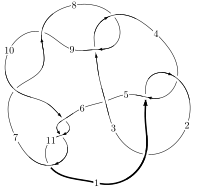
\includegraphics[width=112pt]{../../../GIT/diagram.site/Diagrams/png/261_11a_12.png}\\
\ \ \ A knot diagram\footnotemark}&
\allowdisplaybreaks
\textbf{Linearized knot diagam} \\
\cline{2-2}
 &
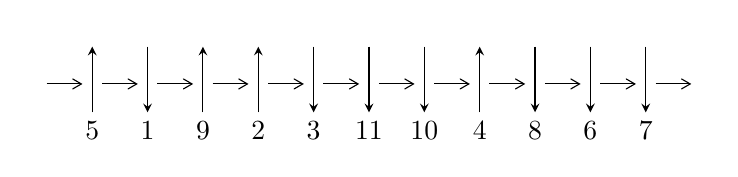
\begin{tikzpicture}[x=20pt, y=17pt]
	% nodes
	\node (C0) at (0, 0) {};
	\node (C1) at (1, 0) {};
	\node (C1U) at (1, +1) {};
	\node (C1D) at (1, -1) {5};

	\node (C2) at (2, 0) {};
	\node (C2U) at (2, +1) {};
	\node (C2D) at (2, -1) {1};

	\node (C3) at (3, 0) {};
	\node (C3U) at (3, +1) {};
	\node (C3D) at (3, -1) {9};

	\node (C4) at (4, 0) {};
	\node (C4U) at (4, +1) {};
	\node (C4D) at (4, -1) {2};

	\node (C5) at (5, 0) {};
	\node (C5U) at (5, +1) {};
	\node (C5D) at (5, -1) {3};

	\node (C6) at (6, 0) {};
	\node (C6U) at (6, +1) {};
	\node (C6D) at (6, -1) {11};

	\node (C7) at (7, 0) {};
	\node (C7U) at (7, +1) {};
	\node (C7D) at (7, -1) {10};

	\node (C8) at (8, 0) {};
	\node (C8U) at (8, +1) {};
	\node (C8D) at (8, -1) {4};

	\node (C9) at (9, 0) {};
	\node (C9U) at (9, +1) {};
	\node (C9D) at (9, -1) {8};

	\node (C10) at (10, 0) {};
	\node (C10U) at (10, +1) {};
	\node (C10D) at (10, -1) {6};

	\node (C11) at (11, 0) {};
	\node (C11U) at (11, +1) {};
	\node (C11D) at (11, -1) {7};
	\node (C12) at (12, 0) {};

	% arrows
	\draw[->,>={angle 60}]
	(C0) edge (C1) (C1) edge (C2) (C2) edge (C3) (C3) edge (C4) (C4) edge (C5) (C5) edge (C6) (C6) edge (C7) (C7) edge (C8) (C8) edge (C9) (C9) edge (C10) (C10) edge (C11) (C11) edge (C12) ;	\draw[->,>=stealth]
	(C1D) edge (C1U) (C2U) edge (C2D) (C3D) edge (C3U) (C4D) edge (C4U) (C5U) edge (C5D) (C6U) edge (C6D) (C7U) edge (C7D) (C8D) edge (C8U) (C9U) edge (C9D) (C10U) edge (C10D) (C11U) edge (C11D) ;
	\end{tikzpicture} \\
\hhline{~~} \\& 
\textbf{Solving Sequence} \\ \cline{2-2} 
 &
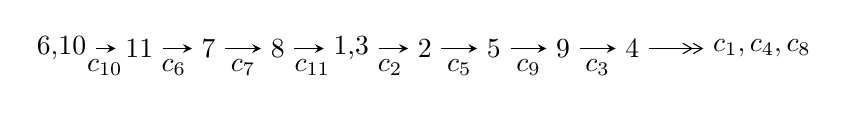
\begin{tikzpicture}[x=25pt, y=7pt]
	% node
	\node (A0) at (-1/8, 0) {6,10};
	\node (A1) at (1, 0) {11};
	\node (A2) at (2, 0) {7};
	\node (A3) at (3, 0) {8};
	\node (A4) at (65/16, 0) {1,3};
	\node (A5) at (41/8, 0) {2};
	\node (A6) at (49/8, 0) {5};
	\node (A7) at (57/8, 0) {9};
	\node (A8) at (65/8, 0) {4};
	\node (C1) at (1/2, -1) {$c_{10}$};
	\node (C2) at (3/2, -1) {$c_{6}$};
	\node (C3) at (5/2, -1) {$c_{7}$};
	\node (C4) at (7/2, -1) {$c_{11}$};
	\node (C5) at (37/8, -1) {$c_{2}$};
	\node (C6) at (45/8, -1) {$c_{5}$};
	\node (C7) at (53/8, -1) {$c_{9}$};
	\node (C8) at (61/8, -1) {$c_{3}$};
	\node (A9) at (10, 0) {$c_{1},c_{4},c_{8}$};

	% edge
	\draw[->,>=stealth]	
	(A0) edge (A1) (A1) edge (A2) (A2) edge (A3) (A3) edge (A4) (A4) edge (A5) (A5) edge (A6) (A6) edge (A7) (A7) edge (A8) ;
	\draw[->>,>={angle 60}]	
	(A8) edge (A9);
\end{tikzpicture} \\ 

\end{tabular} \\

\footnotetext{
The image of knot diagram is generated by the software ``\textbf{Draw programme}" developed by Andrew Bartholomew(\url{http://www.layer8.co.uk/maths/draw/index.htm\#Running-draw}), where we modified some parts for our purpose(\url{https://github.com/CATsTAILs/LinksPainter}).
}\phantom \\ \newline 
\centering \textbf{Ideals for irreducible components\footnotemark of $X_{\text{par}}$} 
 
\begin{align*}
I^u_{1}&=\langle 
5 u^{52}-9 u^{51}+\cdots+b-4,\;5 u^{52}-8 u^{51}+\cdots+2 a-5,\;u^{53}-3 u^{52}+\cdots+6 u^2+1\rangle \\
I^u_{2}&=\langle 
b,\;a^2+a+1,\;u+1\rangle \\
\\
\end{align*}
\raggedright * 2 irreducible components of $\dim_{\mathbb{C}}=0$, with total 55 representations.\\
\footnotetext{All coefficients of polynomials are rational numbers. But the coefficients are sometimes approximated in decimal forms when there is not enough margin.}
\newpage
\renewcommand{\arraystretch}{1}
\centering \section*{I. $I^u_{1}= \langle 5 u^{52}-9 u^{51}+\cdots+b-4,\;5 u^{52}-8 u^{51}+\cdots+2 a-5,\;u^{53}-3 u^{52}+\cdots+6 u^2+1 \rangle$}
\flushleft \textbf{(i) Arc colorings}\\
\begin{tabular}{m{7pt} m{180pt} m{7pt} m{180pt} }
\flushright $a_{6}=$&$\begin{pmatrix}0\\u\end{pmatrix}$ \\
\flushright $a_{10}=$&$\begin{pmatrix}1\\0\end{pmatrix}$ \\
\flushright $a_{11}=$&$\begin{pmatrix}1\\u^2\end{pmatrix}$ \\
\flushright $a_{7}=$&$\begin{pmatrix}- u\\- u^3+u\end{pmatrix}$ \\
\flushright $a_{8}=$&$\begin{pmatrix}u^3-2 u\\- u^3+u\end{pmatrix}$ \\
\flushright $a_{1}=$&$\begin{pmatrix}- u^2+1\\- u^4+2 u^2\end{pmatrix}$ \\
\flushright $a_{3}=$&$\begin{pmatrix}-\frac{5}{2} u^{52}+4 u^{51}+\cdots+\frac{1}{2} u+\frac{5}{2}\\-5 u^{52}+9 u^{51}+\cdots+3 u+4\end{pmatrix}$ \\
\flushright $a_{2}=$&$\begin{pmatrix}-\frac{9}{2} u^{52}+8 u^{51}+\cdots+\frac{5}{2} u+\frac{9}{2}\\-\frac{1}{2} u^{52}+u^{51}+\cdots+\frac{1}{2} u+\frac{1}{2}\end{pmatrix}$ \\
\flushright $a_{5}=$&$\begin{pmatrix}\frac{1}{2} u^{52}- u^{51}+\cdots+\frac{11}{2} u+\frac{1}{2}\\u^{16}-6 u^{14}+\cdots-6 u^3-4 u^2\end{pmatrix}$ \\
\flushright $a_{9}=$&$\begin{pmatrix}u^6-3 u^4+2 u^2+1\\- u^6+2 u^4- u^2\end{pmatrix}$ \\
\flushright $a_{4}=$&$\begin{pmatrix}-\frac{11}{2} u^{52}+10 u^{51}+\cdots+\frac{5}{2} u+\frac{9}{2}\\2 u^{52}-3 u^{51}+\cdots- u-1\end{pmatrix}$\\ \flushright $a_{4}=$&$\begin{pmatrix}-\frac{11}{2} u^{52}+10 u^{51}+\cdots+\frac{5}{2} u+\frac{9}{2}\\2 u^{52}-3 u^{51}+\cdots- u-1\end{pmatrix}$\\&\end{tabular}
\flushleft \textbf{(ii) Obstruction class $= -1$}\\~\\
\flushleft \textbf{(iii) Cusp Shapes $= 11 u^{52}-15 u^{51}+\cdots-11 u-8$}\\~\\
\newpage\renewcommand{\arraystretch}{1}
\flushleft \textbf{(iv) u-Polynomials at the component}\newline \\
\begin{tabular}{m{50pt}|m{274pt}}
Crossings & \hspace{64pt}u-Polynomials at each crossing \\
\hline $$\begin{aligned}c_{1},c_{4}\end{aligned}$$&$\begin{aligned}
&u^{53}+2 u^{52}+\cdots-3 u-1
\end{aligned}$\\
\hline $$\begin{aligned}c_{2}\end{aligned}$$&$\begin{aligned}
&u^{53}+24 u^{52}+\cdots+u-1
\end{aligned}$\\
\hline $$\begin{aligned}c_{3},c_{8}\end{aligned}$$&$\begin{aligned}
&u^{53}+u^{52}+\cdots+12 u+4
\end{aligned}$\\
\hline $$\begin{aligned}c_{5}\end{aligned}$$&$\begin{aligned}
&u^{53}-2 u^{52}+\cdots+5 u-1
\end{aligned}$\\
\hline $$\begin{aligned}c_{6},c_{10},c_{11}\end{aligned}$$&$\begin{aligned}
&u^{53}-3 u^{52}+\cdots+6 u^2+1
\end{aligned}$\\
\hline $$\begin{aligned}c_{7},c_{9}\end{aligned}$$&$\begin{aligned}
&u^{53}+15 u^{52}+\cdots-120 u-16
\end{aligned}$\\
\hline
\end{tabular}\\~\\
\newpage\renewcommand{\arraystretch}{1}
\flushleft \textbf{(v) Riley Polynomials at the component}\newline \\
\begin{tabular}{m{50pt}|m{274pt}}
Crossings & \hspace{64pt}Riley Polynomials at each crossing \\
\hline $$\begin{aligned}c_{1},c_{4}\end{aligned}$$&$\begin{aligned}
&y^{53}+24 y^{52}+\cdots+y-1
\end{aligned}$\\
\hline $$\begin{aligned}c_{2}\end{aligned}$$&$\begin{aligned}
&y^{53}+12 y^{52}+\cdots+25 y-1
\end{aligned}$\\
\hline $$\begin{aligned}c_{3},c_{8}\end{aligned}$$&$\begin{aligned}
&y^{53}+15 y^{52}+\cdots-120 y-16
\end{aligned}$\\
\hline $$\begin{aligned}c_{5}\end{aligned}$$&$\begin{aligned}
&y^{53}+50 y^{51}+\cdots+49 y-1
\end{aligned}$\\
\hline $$\begin{aligned}c_{6},c_{10},c_{11}\end{aligned}$$&$\begin{aligned}
&y^{53}-43 y^{52}+\cdots-12 y-1
\end{aligned}$\\
\hline $$\begin{aligned}c_{7},c_{9}\end{aligned}$$&$\begin{aligned}
&y^{53}+43 y^{52}+\cdots-1248 y-256
\end{aligned}$\\
\hline
\end{tabular}\\~\\
\newpage\flushleft \textbf{(vi) Complex Volumes and Cusp Shapes}
$$\begin{array}{c|c|c}  
\text{Solutions to }I^u_{1}& \I (\text{vol} + \sqrt{-1}CS) & \text{Cusp shape}\\
 \hline 
\begin{aligned}
u &= -0.968116 + 0.283551 I \\
a &= -0.381885 + 0.265140 I \\
b &= \phantom{-}0.072613 - 0.438240 I\end{aligned}
 & -2.32930 + 1.08642 I & -8.77370 + 0.57725 I \\ \hline\begin{aligned}
u &= -0.968116 - 0.283551 I \\
a &= -0.381885 - 0.265140 I \\
b &= \phantom{-}0.072613 + 0.438240 I\end{aligned}
 & -2.32930 - 1.08642 I & -8.77370 - 0.57725 I \\ \hline\begin{aligned}
u &= -0.108156 + 0.876063 I \\
a &= -1.32408 - 1.36471 I \\
b &= \phantom{-}1.61654 + 1.16042 I\end{aligned}
 & \phantom{-}3.78899 + 9.71652 I & -1.28115 - 7.65601 I \\ \hline\begin{aligned}
u &= -0.108156 - 0.876063 I \\
a &= -1.32408 + 1.36471 I \\
b &= \phantom{-}1.61654 - 1.16042 I\end{aligned}
 & \phantom{-}3.78899 - 9.71652 I & -1.28115 + 7.65601 I \\ \hline\begin{aligned}
u &= -0.082170 + 0.858832 I \\
a &= \phantom{-}1.44862 + 0.76672 I \\
b &= -1.73090 - 0.73690 I\end{aligned}
 & \phantom{-}5.69104 + 4.47611 I & \phantom{-}1.74448 - 3.16326 I \\ \hline\begin{aligned}
u &= -0.082170 - 0.858832 I \\
a &= \phantom{-}1.44862 - 0.76672 I \\
b &= -1.73090 + 0.73690 I\end{aligned}
 & \phantom{-}5.69104 - 4.47611 I & \phantom{-}1.74448 + 3.16326 I \\ \hline\begin{aligned}
u &= -0.007145 + 0.820800 I \\
a &= \phantom{-}1.52444 - 0.74981 I \\
b &= -1.84453 + 0.32226 I\end{aligned}
 & \phantom{-}6.01459 + 1.53976 I & \phantom{-}2.52644 - 2.51375 I \\ \hline\begin{aligned}
u &= -0.007145 - 0.820800 I \\
a &= \phantom{-}1.52444 + 0.74981 I \\
b &= -1.84453 - 0.32226 I\end{aligned}
 & \phantom{-}6.01459 - 1.53976 I & \phantom{-}2.52644 + 2.51375 I \\ \hline\begin{aligned}
u &= -1.18911\phantom{ +0.000000I} \\
a &= -0.404114\phantom{ +0.000000I} \\
b &= \phantom{-}1.21704\phantom{ +0.000000I}\end{aligned}
 & -2.34833\phantom{ +0.000000I} & \phantom{-0.000000 } 0 \\ \hline\begin{aligned}
u &= \phantom{-}0.031004 + 0.805221 I \\
a &= -1.40526 + 1.45329 I \\
b &= \phantom{-}1.78482 - 0.80414 I\end{aligned}
 & \phantom{-}4.38710 - 3.67589 I & \phantom{-}0.16278 + 2.56525 I\\
 \hline 
 \end{array}$$\newpage$$\begin{array}{c|c|c}  
\text{Solutions to }I^u_{1}& \I (\text{vol} + \sqrt{-1}CS) & \text{Cusp shape}\\
 \hline 
\begin{aligned}
u &= \phantom{-}0.031004 - 0.805221 I \\
a &= -1.40526 - 1.45329 I \\
b &= \phantom{-}1.78482 + 0.80414 I\end{aligned}
 & \phantom{-}4.38710 + 3.67589 I & \phantom{-}0.16278 - 2.56525 I \\ \hline\begin{aligned}
u &= -0.108842 + 0.774169 I \\
a &= -0.215748 - 0.202638 I \\
b &= \phantom{-}0.884831 + 0.268769 I\end{aligned}
 & \phantom{-}0.49494 + 2.64295 I & -4.27164 - 3.21466 I \\ \hline\begin{aligned}
u &= -0.108842 - 0.774169 I \\
a &= -0.215748 + 0.202638 I \\
b &= \phantom{-}0.884831 - 0.268769 I\end{aligned}
 & \phantom{-}0.49494 - 2.64295 I & -4.27164 + 3.21466 I \\ \hline\begin{aligned}
u &= \phantom{-}1.226730 + 0.035206 I \\
a &= -0.322557 - 1.040730 I \\
b &= \phantom{-}0.081070 - 0.587091 I\end{aligned}
 & -2.80413 - 2.50478 I & \phantom{-0.000000 } 0 \\ \hline\begin{aligned}
u &= \phantom{-}1.226730 - 0.035206 I \\
a &= -0.322557 + 1.040730 I \\
b &= \phantom{-}0.081070 + 0.587091 I\end{aligned}
 & -2.80413 + 2.50478 I & \phantom{-0.000000 } 0 \\ \hline\begin{aligned}
u &= -0.616308 + 0.457732 I \\
a &= -0.500886 - 1.035960 I \\
b &= \phantom{-}0.030166 + 0.720650 I\end{aligned}
 & -3.24252 - 1.36437 I & -10.10455 + 0.49514 I \\ \hline\begin{aligned}
u &= -0.616308 - 0.457732 I \\
a &= -0.500886 + 1.035960 I \\
b &= \phantom{-}0.030166 - 0.720650 I\end{aligned}
 & -3.24252 + 1.36437 I & -10.10455 - 0.49514 I \\ \hline\begin{aligned}
u &= -1.163700 + 0.443994 I \\
a &= -0.632507 - 1.100300 I \\
b &= -1.092410 + 0.318801 I\end{aligned}
 & \phantom{-}0.55249 - 5.00025 I & \phantom{-0.000000 } 0 \\ \hline\begin{aligned}
u &= -1.163700 - 0.443994 I \\
a &= -0.632507 + 1.100300 I \\
b &= -1.092410 - 0.318801 I\end{aligned}
 & \phantom{-}0.55249 + 5.00025 I & \phantom{-0.000000 } 0 \\ \hline\begin{aligned}
u &= -1.218450 + 0.268078 I \\
a &= \phantom{-}0.170099 + 0.071272 I \\
b &= -0.35378 - 1.55230 I\end{aligned}
 & -2.73834 + 1.08871 I & \phantom{-0.000000 } 0\\
 \hline 
 \end{array}$$\newpage$$\begin{array}{c|c|c}  
\text{Solutions to }I^u_{1}& \I (\text{vol} + \sqrt{-1}CS) & \text{Cusp shape}\\
 \hline 
\begin{aligned}
u &= -1.218450 - 0.268078 I \\
a &= \phantom{-}0.170099 - 0.071272 I \\
b &= -0.35378 + 1.55230 I\end{aligned}
 & -2.73834 - 1.08871 I & \phantom{-0.000000 } 0 \\ \hline\begin{aligned}
u &= -1.191390 + 0.413451 I \\
a &= \phantom{-}0.165753 + 1.023680 I \\
b &= \phantom{-}1.384980 + 0.151319 I\end{aligned}
 & \phantom{-}2.28411 + 0.08613 I & \phantom{-0.000000 } 0 \\ \hline\begin{aligned}
u &= -1.191390 - 0.413451 I \\
a &= \phantom{-}0.165753 - 1.023680 I \\
b &= \phantom{-}1.384980 - 0.151319 I\end{aligned}
 & \phantom{-}2.28411 - 0.08613 I & \phantom{-0.000000 } 0 \\ \hline\begin{aligned}
u &= -0.430093 + 0.598904 I \\
a &= -1.44144 - 0.66547 I \\
b &= \phantom{-}0.441095 + 0.500611 I\end{aligned}
 & -2.63045 + 5.30697 I & -7.17193 - 8.38740 I \\ \hline\begin{aligned}
u &= -0.430093 - 0.598904 I \\
a &= -1.44144 + 0.66547 I \\
b &= \phantom{-}0.441095 - 0.500611 I\end{aligned}
 & -2.63045 - 5.30697 I & -7.17193 + 8.38740 I \\ \hline\begin{aligned}
u &= \phantom{-}1.244290 + 0.351593 I \\
a &= -0.585410 + 1.135750 I \\
b &= -1.101840 + 0.108048 I\end{aligned}
 & \phantom{-}0.641453 - 0.489898 I & \phantom{-0.000000 } 0 \\ \hline\begin{aligned}
u &= \phantom{-}1.244290 - 0.351593 I \\
a &= -0.585410 - 1.135750 I \\
b &= -1.101840 - 0.108048 I\end{aligned}
 & \phantom{-}0.641453 + 0.489898 I & \phantom{-0.000000 } 0 \\ \hline\begin{aligned}
u &= -1.294170 + 0.057870 I \\
a &= \phantom{-}0.733580 - 0.333474 I \\
b &= -2.30447 + 0.90915 I\end{aligned}
 & -4.79813 + 3.38896 I & \phantom{-0.000000 } 0 \\ \hline\begin{aligned}
u &= -1.294170 - 0.057870 I \\
a &= \phantom{-}0.733580 + 0.333474 I \\
b &= -2.30447 - 0.90915 I\end{aligned}
 & -4.79813 - 3.38896 I & \phantom{-0.000000 } 0 \\ \hline\begin{aligned}
u &= -1.262360 + 0.367119 I \\
a &= -0.757803 + 0.671105 I \\
b &= \phantom{-}1.92362 + 1.39721 I\end{aligned}
 & \phantom{-}2.12308 + 2.73219 I & \phantom{-0.000000 } 0\\
 \hline 
 \end{array}$$\newpage$$\begin{array}{c|c|c}  
\text{Solutions to }I^u_{1}& \I (\text{vol} + \sqrt{-1}CS) & \text{Cusp shape}\\
 \hline 
\begin{aligned}
u &= -1.262360 - 0.367119 I \\
a &= -0.757803 - 0.671105 I \\
b &= \phantom{-}1.92362 - 1.39721 I\end{aligned}
 & \phantom{-}2.12308 - 2.73219 I & \phantom{-0.000000 } 0 \\ \hline\begin{aligned}
u &= \phantom{-}1.273870 + 0.366638 I \\
a &= \phantom{-}0.073628 - 1.101770 I \\
b &= \phantom{-}1.35653 - 0.53361 I\end{aligned}
 & \phantom{-}2.03469 - 5.80979 I & \phantom{-0.000000 } 0 \\ \hline\begin{aligned}
u &= \phantom{-}1.273870 - 0.366638 I \\
a &= \phantom{-}0.073628 + 1.101770 I \\
b &= \phantom{-}1.35653 + 0.53361 I\end{aligned}
 & \phantom{-}2.03469 + 5.80979 I & \phantom{-0.000000 } 0 \\ \hline\begin{aligned}
u &= -1.291970 + 0.356069 I \\
a &= \phantom{-}1.120780 - 0.449943 I \\
b &= -2.13237 - 2.00334 I\end{aligned}
 & \phantom{-}0.26166 + 7.85803 I & \phantom{-0.000000 } 0 \\ \hline\begin{aligned}
u &= -1.291970 - 0.356069 I \\
a &= \phantom{-}1.120780 + 0.449943 I \\
b &= -2.13237 + 2.00334 I\end{aligned}
 & \phantom{-}0.26166 - 7.85803 I & \phantom{-0.000000 } 0 \\ \hline\begin{aligned}
u &= \phantom{-}1.355440 + 0.136049 I \\
a &= -0.753075 - 0.237855 I \\
b &= \phantom{-}0.928079 - 0.540827 I\end{aligned}
 & -5.74714 - 3.41063 I & \phantom{-0.000000 } 0 \\ \hline\begin{aligned}
u &= \phantom{-}1.355440 - 0.136049 I \\
a &= -0.753075 + 0.237855 I \\
b &= \phantom{-}0.928079 + 0.540827 I\end{aligned}
 & -5.74714 + 3.41063 I & \phantom{-0.000000 } 0 \\ \hline\begin{aligned}
u &= \phantom{-}1.333880 + 0.341289 I \\
a &= \phantom{-}0.269451 + 0.152167 I \\
b &= -0.70513 + 1.50804 I\end{aligned}
 & -4.03348 - 6.68828 I & \phantom{-0.000000 } 0 \\ \hline\begin{aligned}
u &= \phantom{-}1.333880 - 0.341289 I \\
a &= \phantom{-}0.269451 - 0.152167 I \\
b &= -0.70513 - 1.50804 I\end{aligned}
 & -4.03348 + 6.68828 I & \phantom{-0.000000 } 0 \\ \hline\begin{aligned}
u &= \phantom{-}1.329340 + 0.384853 I \\
a &= -0.862126 - 0.636182 I \\
b &= \phantom{-}1.64046 - 1.66007 I\end{aligned}
 & \phantom{-}1.26818 - 8.94141 I & \phantom{-0.000000 } 0\\
 \hline 
 \end{array}$$\newpage$$\begin{array}{c|c|c}  
\text{Solutions to }I^u_{1}& \I (\text{vol} + \sqrt{-1}CS) & \text{Cusp shape}\\
 \hline 
\begin{aligned}
u &= \phantom{-}1.329340 - 0.384853 I \\
a &= -0.862126 + 0.636182 I \\
b &= \phantom{-}1.64046 + 1.66007 I\end{aligned}
 & \phantom{-}1.26818 + 8.94141 I & \phantom{-0.000000 } 0 \\ \hline\begin{aligned}
u &= \phantom{-}1.398170 + 0.082873 I \\
a &= \phantom{-}0.626703 - 0.081349 I \\
b &= -0.96603 + 1.31820 I\end{aligned}
 & -9.55416 - 0.10492 I & \phantom{-0.000000 } 0 \\ \hline\begin{aligned}
u &= \phantom{-}1.398170 - 0.082873 I \\
a &= \phantom{-}0.626703 + 0.081349 I \\
b &= -0.96603 - 1.31820 I\end{aligned}
 & -9.55416 + 0.10492 I & \phantom{-0.000000 } 0 \\ \hline\begin{aligned}
u &= \phantom{-}1.347190 + 0.390740 I \\
a &= \phantom{-}1.171490 + 0.397318 I \\
b &= -1.70731 + 2.12421 I\end{aligned}
 & -0.7808 - 14.2618 I & \phantom{-0.000000 } 0 \\ \hline\begin{aligned}
u &= \phantom{-}1.347190 - 0.390740 I \\
a &= \phantom{-}1.171490 - 0.397318 I \\
b &= -1.70731 - 2.12421 I\end{aligned}
 & -0.7808 + 14.2618 I & \phantom{-0.000000 } 0 \\ \hline\begin{aligned}
u &= \phantom{-}1.397480 + 0.165043 I \\
a &= \phantom{-}0.932544 + 0.257510 I \\
b &= -1.53992 + 0.33246 I\end{aligned}
 & -8.47430 - 7.85966 I & \phantom{-0.000000 } 0 \\ \hline\begin{aligned}
u &= \phantom{-}1.397480 - 0.165043 I \\
a &= \phantom{-}0.932544 - 0.257510 I \\
b &= -1.53992 - 0.33246 I\end{aligned}
 & -8.47430 + 7.85966 I & \phantom{-0.000000 } 0 \\ \hline\begin{aligned}
u &= -0.340173 + 0.453801 I \\
a &= \phantom{-}1.060390 + 0.375276 I \\
b &= -0.159985 - 0.452155 I\end{aligned}
 & -0.42373 + 1.39478 I & -2.79014 - 5.25225 I \\ \hline\begin{aligned}
u &= -0.340173 - 0.453801 I \\
a &= \phantom{-}1.060390 - 0.375276 I \\
b &= -0.159985 + 0.452155 I\end{aligned}
 & -0.42373 - 1.39478 I & -2.79014 + 5.25225 I \\ \hline\begin{aligned}
u &= \phantom{-}0.020226 + 0.357518 I \\
a &= \phantom{-}2.02061 + 0.44390 I \\
b &= -0.218240 - 0.573207 I\end{aligned}
 & \phantom{-}0.51548 + 1.38171 I & \phantom{-}2.20295 - 4.47540 I\\
 \hline 
 \end{array}$$\newpage$$\begin{array}{c|c|c}  
\text{Solutions to }I^u_{1}& \I (\text{vol} + \sqrt{-1}CS) & \text{Cusp shape}\\
 \hline 
\begin{aligned}
u &= \phantom{-}0.020226 - 0.357518 I \\
a &= \phantom{-}2.02061 - 0.44390 I \\
b &= -0.218240 + 0.573207 I\end{aligned}
 & \phantom{-}0.51548 - 1.38171 I & \phantom{-}2.20295 + 4.47540 I \\ \hline\begin{aligned}
u &= \phantom{-}0.219966 + 0.200182 I \\
a &= -3.43324 - 0.35025 I \\
b &= \phantom{-}0.603600 + 0.354674 I\end{aligned}
 & -0.24387 - 2.48522 I & \phantom{-}1.64376 + 3.61634 I \\ \hline\begin{aligned}
u &= \phantom{-}0.219966 - 0.200182 I \\
a &= -3.43324 + 0.35025 I \\
b &= \phantom{-}0.603600 - 0.354674 I\end{aligned}
 & -0.24387 + 2.48522 I & \phantom{-}1.64376 - 3.61634 I\\
 \hline 
 \end{array}$$\newpage\newpage\renewcommand{\arraystretch}{1}
\centering \section*{II. $I^u_{2}= \langle b,\;a^2+a+1,\;u+1 \rangle$}
\flushleft \textbf{(i) Arc colorings}\\
\begin{tabular}{m{7pt} m{180pt} m{7pt} m{180pt} }
\flushright $a_{6}=$&$\begin{pmatrix}0\\-1\end{pmatrix}$ \\
\flushright $a_{10}=$&$\begin{pmatrix}1\\0\end{pmatrix}$ \\
\flushright $a_{11}=$&$\begin{pmatrix}1\\1\end{pmatrix}$ \\
\flushright $a_{7}=$&$\begin{pmatrix}1\\0\end{pmatrix}$ \\
\flushright $a_{8}=$&$\begin{pmatrix}1\\0\end{pmatrix}$ \\
\flushright $a_{1}=$&$\begin{pmatrix}0\\1\end{pmatrix}$ \\
\flushright $a_{3}=$&$\begin{pmatrix}a\\0\end{pmatrix}$ \\
\flushright $a_{2}=$&$\begin{pmatrix}a\\- a\end{pmatrix}$ \\
\flushright $a_{5}=$&$\begin{pmatrix}a+1\\-1\end{pmatrix}$ \\
\flushright $a_{9}=$&$\begin{pmatrix}1\\0\end{pmatrix}$ \\
\flushright $a_{4}=$&$\begin{pmatrix}a\\0\end{pmatrix}$\\ \flushright $a_{4}=$&$\begin{pmatrix}a\\0\end{pmatrix}$\\&\end{tabular}
\flushleft \textbf{(ii) Obstruction class $= 1$}\\~\\
\flushleft \textbf{(iii) Cusp Shapes $= -4 a-5$}\\~\\
\newpage\renewcommand{\arraystretch}{1}
\flushleft \textbf{(iv) u-Polynomials at the component}\newline \\
\begin{tabular}{m{50pt}|m{274pt}}
Crossings & \hspace{64pt}u-Polynomials at each crossing \\
\hline $$\begin{aligned}c_{1},c_{2},c_{5}\end{aligned}$$&$\begin{aligned}
&u^2+u+1
\end{aligned}$\\
\hline $$\begin{aligned}c_{3},c_{7},c_{8}\\c_{9}\end{aligned}$$&$\begin{aligned}
&u^2
\end{aligned}$\\
\hline $$\begin{aligned}c_{4}\end{aligned}$$&$\begin{aligned}
&u^2- u+1
\end{aligned}$\\
\hline $$\begin{aligned}c_{6}\end{aligned}$$&$\begin{aligned}
&(u-1)^2
\end{aligned}$\\
\hline $$\begin{aligned}c_{10},c_{11}\end{aligned}$$&$\begin{aligned}
&(u+1)^2
\end{aligned}$\\
\hline
\end{tabular}\\~\\
\newpage\renewcommand{\arraystretch}{1}
\flushleft \textbf{(v) Riley Polynomials at the component}\newline \\
\begin{tabular}{m{50pt}|m{274pt}}
Crossings & \hspace{64pt}Riley Polynomials at each crossing \\
\hline $$\begin{aligned}c_{1},c_{2},c_{4}\\c_{5}\end{aligned}$$&$\begin{aligned}
&y^2+y+1
\end{aligned}$\\
\hline $$\begin{aligned}c_{3},c_{7},c_{8}\\c_{9}\end{aligned}$$&$\begin{aligned}
&y^2
\end{aligned}$\\
\hline $$\begin{aligned}c_{6},c_{10},c_{11}\end{aligned}$$&$\begin{aligned}
&(y-1)^2
\end{aligned}$\\
\hline
\end{tabular}\\~\\
\newpage\flushleft \textbf{(vi) Complex Volumes and Cusp Shapes}
$$\begin{array}{c|c|c}  
\text{Solutions to }I^u_{2}& \I (\text{vol} + \sqrt{-1}CS) & \text{Cusp shape}\\
 \hline 
\begin{aligned}
u &= -1.00000\phantom{ +0.000000I} \\
a &= -0.500000 + 0.866025 I \\
b &= \phantom{-0.000000 } 0\end{aligned}
 & -1.64493 + 2.02988 I & -3.00000 - 3.46410 I \\ \hline\begin{aligned}
u &= -1.00000\phantom{ +0.000000I} \\
a &= -0.500000 - 0.866025 I \\
b &= \phantom{-0.000000 } 0\end{aligned}
 & -1.64493 - 2.02988 I & -3.00000 + 3.46410 I\\
 \hline 
 \end{array}$$\newpage
\newpage\renewcommand{\arraystretch}{1}
\centering \section*{ III. u-Polynomials}
\begin{tabular}{m{50pt}|m{274pt}}
Crossings & \hspace{64pt}u-Polynomials at each crossing \\
\hline $$\begin{aligned}c_{1}\end{aligned}$$&$\begin{aligned}
&(u^2+u+1)(u^{53}+2 u^{52}+\cdots-3 u-1)
\end{aligned}$\\
\hline $$\begin{aligned}c_{2}\end{aligned}$$&$\begin{aligned}
&(u^2+u+1)(u^{53}+24 u^{52}+\cdots+u-1)
\end{aligned}$\\
\hline $$\begin{aligned}c_{3},c_{8}\end{aligned}$$&$\begin{aligned}
&u^2(u^{53}+u^{52}+\cdots+12 u+4)
\end{aligned}$\\
\hline $$\begin{aligned}c_{4}\end{aligned}$$&$\begin{aligned}
&(u^2- u+1)(u^{53}+2 u^{52}+\cdots-3 u-1)
\end{aligned}$\\
\hline $$\begin{aligned}c_{5}\end{aligned}$$&$\begin{aligned}
&(u^2+u+1)(u^{53}-2 u^{52}+\cdots+5 u-1)
\end{aligned}$\\
\hline $$\begin{aligned}c_{6}\end{aligned}$$&$\begin{aligned}
&((u-1)^2)(u^{53}-3 u^{52}+\cdots+6 u^2+1)
\end{aligned}$\\
\hline $$\begin{aligned}c_{7},c_{9}\end{aligned}$$&$\begin{aligned}
&u^2(u^{53}+15 u^{52}+\cdots-120 u-16)
\end{aligned}$\\
\hline $$\begin{aligned}c_{10},c_{11}\end{aligned}$$&$\begin{aligned}
&((u+1)^2)(u^{53}-3 u^{52}+\cdots+6 u^2+1)
\end{aligned}$\\
\hline
\end{tabular}\newpage\renewcommand{\arraystretch}{1}
\centering \section*{ IV. Riley Polynomials}
\begin{tabular}{m{50pt}|m{274pt}}
Crossings & \hspace{64pt}Riley Polynomials at each crossing \\
\hline $$\begin{aligned}c_{1},c_{4}\end{aligned}$$&$\begin{aligned}
&(y^2+y+1)(y^{53}+24 y^{52}+\cdots+y-1)
\end{aligned}$\\
\hline $$\begin{aligned}c_{2}\end{aligned}$$&$\begin{aligned}
&(y^2+y+1)(y^{53}+12 y^{52}+\cdots+25 y-1)
\end{aligned}$\\
\hline $$\begin{aligned}c_{3},c_{8}\end{aligned}$$&$\begin{aligned}
&y^2(y^{53}+15 y^{52}+\cdots-120 y-16)
\end{aligned}$\\
\hline $$\begin{aligned}c_{5}\end{aligned}$$&$\begin{aligned}
&(y^2+y+1)(y^{53}+50 y^{51}+\cdots+49 y-1)
\end{aligned}$\\
\hline $$\begin{aligned}c_{6},c_{10},c_{11}\end{aligned}$$&$\begin{aligned}
&((y-1)^2)(y^{53}-43 y^{52}+\cdots-12 y-1)
\end{aligned}$\\
\hline $$\begin{aligned}c_{7},c_{9}\end{aligned}$$&$\begin{aligned}
&y^2(y^{53}+43 y^{52}+\cdots-1248 y-256)
\end{aligned}$\\
\hline
\end{tabular}
\vskip 2pc
\end{document}